% !TEX root = SocialVision2012.tex

\subsection{Datasets and Challenge Problems}
\label{sec:sys}

\begin{figure}[t!]
\begin{center}
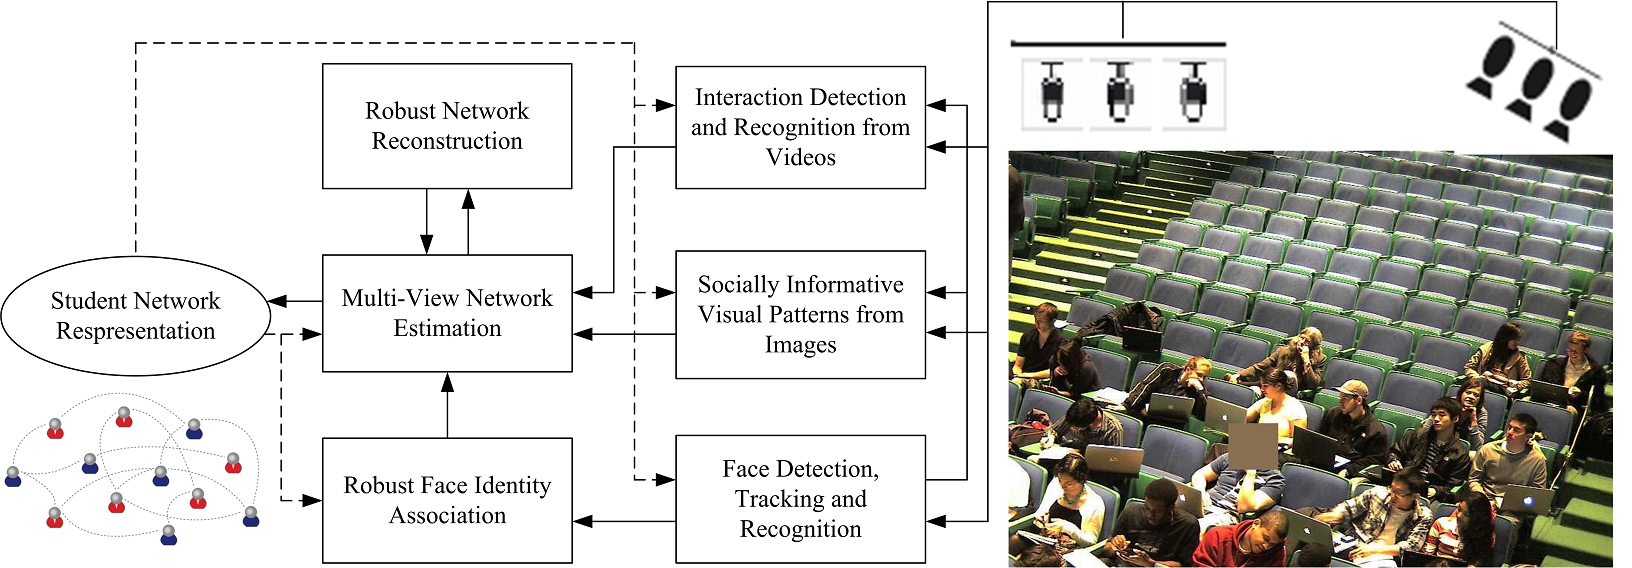
\includegraphics[width=\columnwidth]{prototype_1}
\end{center}
\vspace{-0.25in} \caption{\captionsize 
The prototype hardware and software infrastructure for analyzing socialized human behaviors in an indoor environment for social network estimation at Harvard University.\todd{Add on the right of this figure an image from UT Interaction dataset (labeled ``severely constrained'') and an image from Grand Central Station (labeled ``unconstrained''). Also add label ``moderately constrained'' above the classroom image.}\label{fig:prototype}\afterfigspace}
\end{figure}

Our goal is to build a foundation for social analysis in diverse, unconstrained environments like that depicted in the bottom-right of Fig.~\ref{fig:prototype}. This is becoming well within reach thanks to the ready availability of networked camera arrays and advances in practical multi-view detection and tracking (e.g.,~\cite{EshelM10}). These unconstrained environments are fundamentally different from scenarios considered in existing benchmark datasets for interaction analysis (top-right of Fig.~\ref{fig:prototype}), where the interactions involve a pre-determined number of participants; take place in the absence of by-standers or social clutter; and/or are localized in time \emph{a priori}~\cite{} \todd{Add citations to UT Interaction dataset and Caltech mouse dataset here. others?}. Because of these  differences, evaluations on existing benchmarks fail to provide meaningful proxies for fundamental progress in large-scale social visual analysis.

As part of the proposed activity, we will create new datasets and challenge problems that make it possible to measure meaningful progress on social visual analysis, and at the same time, serve as a mechanism to engage the broader computer vision research community. To ensure that our benchmarks provide effective measures of progress, they will be annotated with ground-truth information about identities, interaction categories, and social relationships. We will create and use two distinct types of datasets. The first type will be based on video collections that are already being collected in large interactive classrooms at Harvard University. These datasets will be large (about \todd{XXX} camera-hours of video have been collected so far) and will enable evaluation of all aspects of the proposed research program, but because of the need for maintaining privacy of the observed subjects they will not be made directly available to non-collaborating research groups. The second type of datasets will supplement the first by being made publicly available. These will be smaller collections of annotated videos that contain interactions staged by informed actors, and they will simulate unconstrained environments by including long videos of large social gatherings. These will enable the evaluation of some aspects of the proposed research program (e.g., detecting interaction categories) and will be presented as ``challenge problems" for the broader computer vision research community.

\subsection{Harvard Interactive Classroom Datasets}
We will leverage video that is currently being collected by camera arrays in large interactive classrooms at Harvard University. These systems, which we collectively call ``Lens to Learning'', have been developed over the past three years with funding by the NSF (IIS-0835338, 2009--2012) and the Harvard Initiative for Learning and Teaching (HILT)\footnote{\href{http://hilt.harvard.edu/2012-2013-awards}{http://hilt.harvard.edu/2012-2013-awards}} with the goal of understanding how students learn in interactive classrooms. The observed classrooms are ``interactive'' in that students frequently engage in ad-hoc discussions. One commonly used technique is \emph{Peer Instruction}, which involves brief student discussions during the time traditionally devoted to lecture. Each discussion begins with a single ConcepTest---a question designed to elicit common student misconceptions [19,70]. The students are given a moment to formulate and electronically submit their individual answer to the question posed, and then they are asked to form ad-hoc discussion groups to try to convince neighboring students of the correctness of their answers. After a few minutes of peer-to-peer discussion, students submit their possibly-revised answers, and this entire activity is usually followed by the instructor�s reinforcement of the main concept. Education research suggests that both high and low ability students benefit from these discussions [24,36,80,83].

The videos collected by Lens to Learning present a unique opportunity for developing and evaluation large-scale social visual analysis. The observed classrooms, including that in the middle of Fig.~\ref{fig:prototype}, contain a hundred or more individuals engaged in ad-hoc interactions. This is fundamentally different from severely constrained environments (top-right Fig.~\ref{fig:prototype}), where interactions are manually pre-localized in space or time. The utility of large classrooms for social visual research stems not only from the number and diversity of people they contain, but from the nature of activities that are exhibited there and the non-visual sources of metadata that are available for evaluation. Individuals typically remain seated and forward-facing, and this simplifies detection and tracking, allowing us to focus our research on the higher-level challenges of reasoning about social interactions and relationships. Through immense effort by educational experts (using techniques like those in [92]), a handful of semantically-meaningful interaction categories have already been discovered in these videos, and occurrences of these interactions have been painstakingly annotated in . Finally, in addition to video data, we have access to many non-visual sources of social network information (educational outcomes, answers to ConcepTests, lab section assignments, etc.) that can be used to cross-validate the social networks produced by our vision-based techniques that we propose to build.

-over the course of a whole semester...

The ultimate goal of our proposed research is a comprehensive system that seamlessly integrates a bottom-up hierarchy of multiple modules for sensing social networks from visual information. While an universally applicable framework or prototype system to accomplish this purpose is a long-term objective that may require more than affordable for the moment, at a reasonably constrained visual scene and a fixed group of social agents of small to medium scale is completely feasible and is on our agenda. We plan, for example, at a later stage of the award period, to move toward such a computer vision system that can reveal the heterogeneous and possibly time-varying social networks of all students that enroll in a semester-long course offered at Harvard University. 

As the initial attempt toward this goal to analyze socialized human behaviors in an indoor environment for social network estimation, we have built up a prototype hardware and software infrastructure at Harvard University. As shown in Fig. \ref{fig:prototype}, the hardware part of the prototype system mainly consists of a networked audio-visual recording system for large-scale recording of student interactions in a Harvard College lecture hall. The system records audio and video from approximately one hundred students during each lecture in conjunction with the audience responses through an online teaching-learning application. The video system uses six IP cameras that together provide resolution that is high enough to achieve face-based identity recognition of each student in the audience. The audio system is an innovative design consisting 48 omnidirectional boundary microphones mounted inconspicuously among the seats, and outputting sound from each microphone recording to a single user-friendly mp3 audio file.To automatically analyze the videos, we have developed a robust computational suite of computer vision tools. This software has consisted of several fundamental modules that detect, track, and recognize faces,  distill socially informative descriptions from raw images, and detect and recognize salient social interactions of interest, and has yielded the data that are fundamentally different from benchmark datasets \cite{UTdata,Choi:context,Choi:recogtrack} and are used for our preliminary evaluation introduction in Section \ref{sec:activity}. The software suits, meanwhile, is expected to include other functionalities proposed in the previous sections by the end of the award period.

As illustrated by the diagram in Fig. \ref{fig:prototype}, and mentioned in the previous sections, we will employ the classroom observation system as our interface to harvest a volume of video sequences recording the indoor behaviors of the same class of students throughout the semester. The course that they enroll in uses interactive instruction by which they students are self-seated and engage in ad-hocly grouped discussions. We also maintain a teaching database where we have textual metadata regarding the students' profile data, status, learning performance, etc., as initial and partial social contexts among the students. This teaching database only only provides extra non-visual sources for estimating the student social network, but also can be used to provide the `ground-truth' networks to facilitate the research proposed in Section \ref{sec:vis2net}. Eventually, through the modules for face detection, tracking, recognition, and identify association (Section \ref{sec:assoc}), we link the members/nodes of the network to the human beings in each scene. Meanwhile, we detect socially meaningful interactions (Section \ref{subsec:activity}), co-occurrences, as well as compute other low-level visual cues for the purpose of estimating a `noisy' version of a multi-view network representation (Section \ref{sec:vis2net}), with the unobservable links between pairs in different views robustly reconstructed(Section \ref{sec:reconstruct}). The `hallucinated' social network from the videos in this way then provides the visually-sensed `honest' update for the network prior and is consolidated with the `textual' network as a comprehensive and more accurate characterization of this community. The feedback channel may infuse the updated social contexts and concepts to the face recognizer and the interaction detector. We expect such a close-loop socially-aware visual analytical framework to learn and self-build themselves in an evolving and unsupervised manner and to enable our new look at the images and videos in this socially networked era.


\subsubsection{Additional data acquisition and challenges}

An encouraging trend in computer vision over the last several years has been the increasing use of benchmark datasets for evaluating progress on particular tasks. Standardized datasets, such as the Middlebury Stereo Evaluation project~\cite{}, the PASCAL VOC Challenges~\cite{}, the Berkeley Segmentation Database~\cite{}, and the KTH database of individual actions~\cite{}, have served as catalysts for progress on difficult problems because they create concrete targets that inspire new ideas and allow researchers to evaluate their systems by quantitatively demonstrating improvement.

Currently, there are relatively few datasets available for problems related to social visual analysis...

Our proposed framework of social visual analytics is directly applicable to other `socialized imageries', such as online photo albums from Facebook or Flickr that we investigated in our previous work \cite{Stone2008,Stone2010}. We expect to employ a similar data acquisition model as introduced in \cite{Stone2008,Stone2010} for collecting complementing datasets from online sources.  In either the data from classroom interactions or materials harvested from online, there has been the challenges regarding privacy conservation and public availability of these materials. The way that we will adopt for prompting resource sharing and reproducible research will be in multiple levels. We will, for example, explore a way for `internal sharing', in which colleague researchers submit their companion prototype software and we evaluate it locally on their behalf. We will also seek to produce `privacy-conserved' version of the data, which can be a subset of the entire database with sensitive elements properly encrypted or removed. Finally and in particular, We will aim to provide new datasets that are free of privacy or publishability concerns, which serve for growing progress in the community with high potential and significant impact.









%With this established classroom observation system and these fundamental modules, we have successfully collected and processed a large-scale classroom behavior database consisting of 100 video clips in total. The students are seated in a regular lecture hall and are observed by a camera array with non-overlapping fields of view. The classroom is ``interactive'' because at various times throughout the lecture students are invited to engage in ad-hoc group discussions about problems provided by the instructor. The scale of our database is orders of magnitude larger than state-of-the-art computer vision datasets (e.g. those used in \cite{UTdata,Choi:context,Choi:recogtrack}), in the number of individuals (10-50 students per camera), the number of cameras (6), and the amount of time (100 minutes per camera, per recording, equaling over 3,000 minutes in total). Through a combination of face detection and tracking, we obtained noisy tracks for all students in each monocular video, upon which we developed descriptive modules that directly extract descriptiors such as head pose and body motion, we have also implemented a high-level module for behavior analysis based on similarity between two social groups, as depicted in Fig. \ref{fig:prototype}(b). In this module, the behavior of each individual is represented by a combination of the head pose and the motion of torso and arms (using the method of histogram of optical flows). The social behavior of a group is then represented by the configuration in space and time of the behaviors of its participants. With this social activity representation, the module detects a salient social activity from a new video and retrieves similar social activities from our established database. This functionality is illustrated in Fig. \ref{fig:prototype}(b), where our system has discovered a three-way conversation by identifying the participants of this conversation and the time span (several to tens of seconds) of this event. Based on the behavior representation for this space-time social interaction, the system searches the remainder of the database and retrieves a list of exemplars containing similar social behavior, ranked in the descending order of the similarities with the query. In this way, any manual annotations associated with the query video can be propagated to the top-ranking exemplars, and we are now taking this approach to propagate our manual annotations across the whole database. 








%At the current and initial stage of the effort to bring socialized semantics to computer vision, it can be usually the case that we do not have sufficient social contexts to help improving our target/face recognition, and we are not always specific about what are the meaningful social interactive activities that are most informative for social description. Conversely, we may neither know clearly about what exactly we should distill from images to fulfill a network learning task, nor have concrete knowledge about how the multiple views or overlapping community structures of a network will eventually turn out to be. However, we have argued at the beginning and demonstrated through the four proposed research problems the fact that the two aspects assist and benefit from each other, and an overall socially-aware visual analytical system is our ultimate goal. To this end, our final proposed research will include an attempt for a framework that eventually integrate social information and image understanding and allow them to learn and self-build themselves in an evolving and unsupervised manner.





